\setcounter{ExampleCounter}{1}
\begin{comment}
\begin{center}
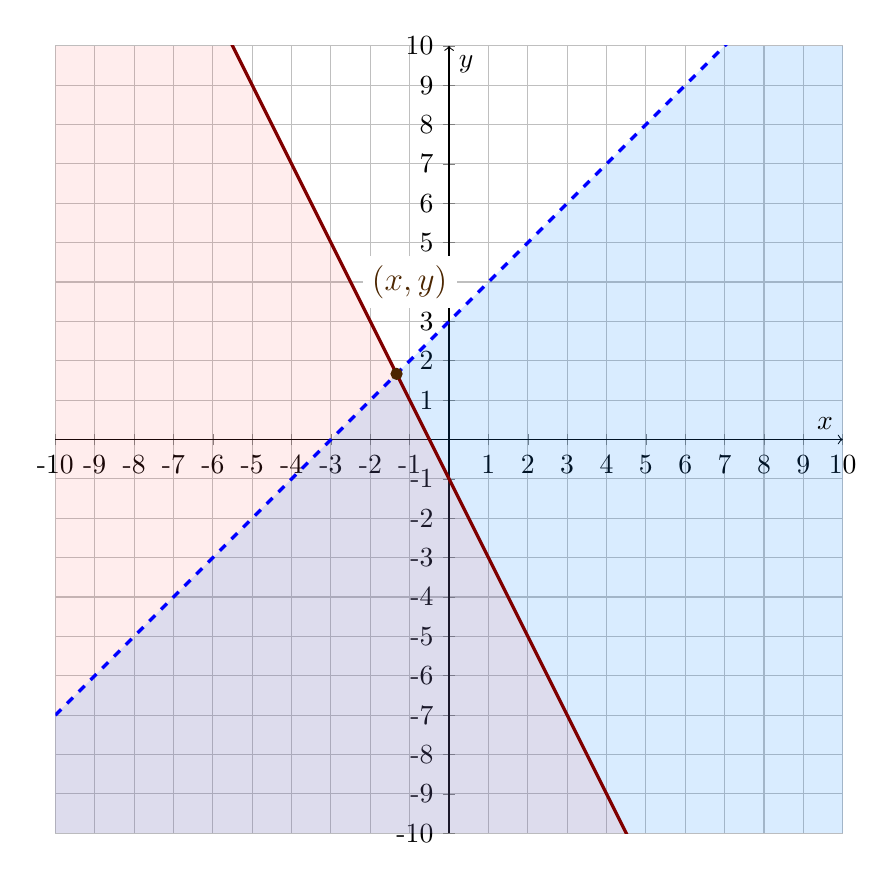
\begin{tikzpicture}
\begin{axis}[
    xmin=-10, xmax=10,
    ymin=-10, ymax=10,
    axis lines=center,
    axis on top=false,
    domain=0:1,
    x=0.5cm,
    y=0.5cm,
    xtick={-10,-9,...,10},
    xticklabels={-10,-9,...,10},
    ytick={-10,-9,...,10},
    yticklabels={-10,-9,...,10},
    axis lines=middle,
    axis line style={->},
    xlabel={$x$},
    ylabel={$y$},
    grid=major
    ]
    \addplot [only marks,color=orange!30!black] table {
	-1.333 1.667
	};
	\addplot [thick,color=blue,fill=blue!50!cyan, 
                    fill opacity=0.15,draw opacity=0]coordinates {
            (7, 10)
            (10,10)
            (10,-10)
            (-10,-10)
            (-10, -7)  };
    \addplot [thick,color=blue,fill=red!70!white, 
                    fill opacity=0.1,draw opacity=0]coordinates {
            (-11/2, 10) 
            (9/2, -10)
            (-10,-10)
            (-10, 10)  };
	\draw [yshift=12.5cm,xshift=4.5cm] node [fill=white] {\large\color{orange!30!black}$(x,y)$};
	\addplot [very thick,blue,dashed,domain=-10:10] {x+3};
	\addplot [very thick,red!50!black,domain=-10:10] {-2*x-1};
\end{axis}
\end{tikzpicture}
\end{center}
\end{comment}

In the application problems that we'll do later in this chapter, we'll come across linear \emph{inequalities}, in addition to linear equations.  Linear inequalities look like the following:
\[2x+9y \leq 3.\]
Let's think about what this says.  This says that whatever $x$ and $y$ are, if we multiply $x$ by 2, multiply $y$ by 9, and add them together, our answer will be smaller than 3 (or equal to 3).  Clearly, this isn't true for \emph{any} choice of $x$ and $y$ (for example, what if $x=100$ and $y=100$?), but the combinations of $x$ and $y$ that fit this inequality are called its \textbf{solution set}, just like the solution set to the equations we saw in the last two sections is the combination of $x$ and $y$ that fit into it and make it true.

When we graphed a linear equation, we found that all the solutions were arranged neatly along a straight line.  We'd like to have a graphical interpretation for the solutions to a linear inequality, as well.  Think of the following simple example:
\[y \leq 2\]
This says that all the points whose $y$-coordinates are 6 or less will be solutions.  If we start plotting all those points, we find that they are all the points that lie below the line $y=2$.
\begin{center}
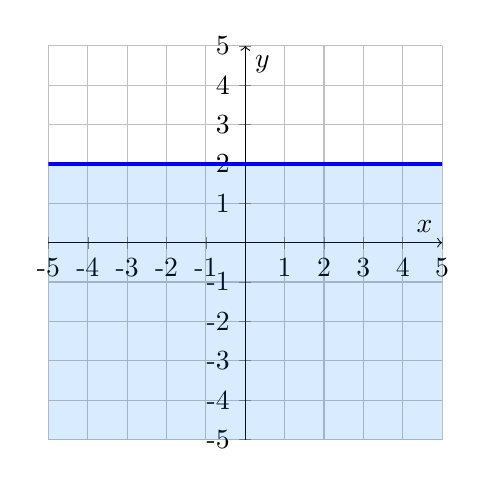
\begin{tikzpicture}
\begin{axis}[
    xmin=-5, xmax=5,
    ymin=-5, ymax=5,
    axis lines=center,
    axis on top=false,
    domain=0:1,
    x=0.5cm,
    y=0.5cm,
    xtick={-10,-9,...,10},
    xticklabels={-10,-9,...,10},
    ytick={-10,-9,...,10},
    yticklabels={-10,-9,...,10},
    axis lines=middle,
    axis line style={->},
    xlabel={$x$},
    ylabel={$y$},
    grid=major
    ]
	\addplot [thick,color=blue,fill=blue!50!cyan, 
                    fill opacity=0.15,draw opacity=0]coordinates {
            (-10,2)
            (10,2)
            (10,-10)
            (-10, -10)  };
	\draw [yshift=12.5cm,xshift=4.5cm] node [fill=white] {\large\color{orange!30!black}$(x,y)$};
	\addplot [very thick,blue,domain=-10:10] {2};
\end{axis}
\end{tikzpicture}
\end{center}

What about another example?
\[x > -1\]
Here, the solution set is all the points whose $x$-coordinate is greater than -1.  However, notice that we are \emph{not} including the points whose $x$-coordinate is equal to -1 (along the line $x=-1$), so we draw the line dashed this time:
\begin{center}
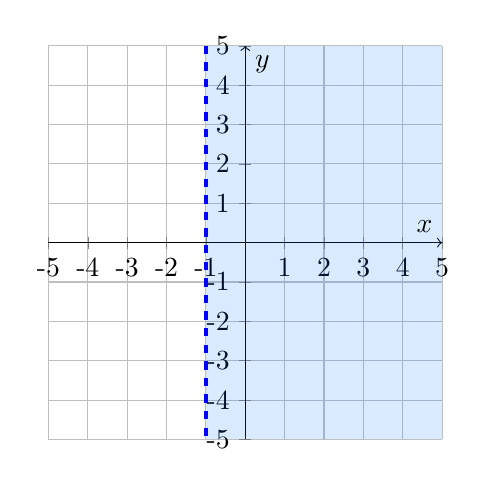
\begin{tikzpicture}
\begin{axis}[
    xmin=-5, xmax=5,
    ymin=-5, ymax=5,
    axis lines=center,
    axis on top=false,
    domain=0:1,
    x=0.5cm,
    y=0.5cm,
    xtick={-10,-9,...,10},
    xticklabels={-10,-9,...,10},
    ytick={-10,-9,...,10},
    yticklabels={-10,-9,...,10},
    axis lines=middle,
    axis line style={->},
    xlabel={$x$},
    ylabel={$y$},
    grid=major
    ]
	\addplot [thick,color=blue,fill=blue!50!cyan, 
                    fill opacity=0.15,draw opacity=0]coordinates {
            (-1,5)
            (-1,-5)
            (5,-5)
            (5, 5)  };
    \draw [very thick,blue,dashed] (2cm,5cm) -- (2cm,0cm);	
\end{axis}
\end{tikzpicture}
\end{center}

These two examples illustrate how we will draw the solution set of a linear inequality.  We can graph a linear inequality by first changing the inequality sign to an equals sign and graphing the resulting line.
\begin{proc}{The Solution Set of a Linear Inequality}
The graph of the solutions to a linear inequality consist of every point to one side of the corresponding line.\\

If the inequality is $\geq$ or $\leq$, we draw the boundary solid, and if the inequality is $>$ or $<$, we draw the boundary dashed.
\end{proc}

Once we've graphed the corresponding line, all we have to do is figure out which side of the line to shade.  The simplest way to do this is to pick a test point on one side of the line and see if it is a solution.  If it is, shade that side; if not, shade the other side.

\begin{example}[https://www.youtube.com/watch?v=Rtp32uyVjzs]{Graphing a Linear Inequality}
Graph the solution set for the following inequality.
\[x-y\leq 1\]

\sol
We begin by graphing the line $x-y=1$ using the intercepts:
\begin{center}
$(1,0)$ and $(0,-1)$
\end{center}
Since the inequality \emph{includes} 1 (it is less than \emph{or equal to}), we draw the line solid.
\begin{center}
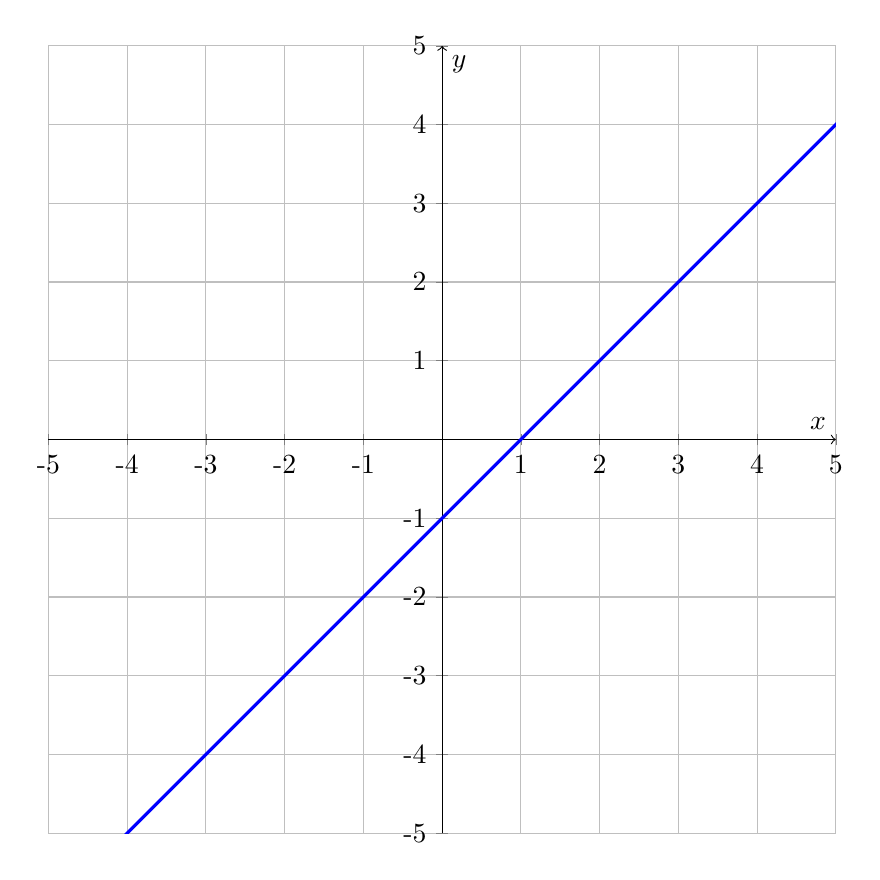
\begin{tikzpicture}
\begin{axis}[
    xmin=-5, xmax=5,
    ymin=-5, ymax=5,
    axis lines=center,
    axis on top=false,
    domain=0:1,
    x=1cm,
    y=1cm,
    xtick={-10,-9,...,10},
    xticklabels={-10,-9,...,10},
    ytick={-10,-9,...,10},
    yticklabels={-10,-9,...,10},
    axis lines=middle,
    axis line style={->},
    xlabel={$x$},
    ylabel={$y$},
    grid=major
    ]
    \addplot [very thick,blue,domain=-10:10] {x-1};	
\end{axis}
\end{tikzpicture}
\end{center}

Now, to figure out which side to shade, we pick a test point.  The simplest is the origin: $(0,0)$.  This is clearly above the line--if it satisfies the inequality, we shade the upper side; if not, we shade the lower side.\\

Check $(0,0)$ in the inequality:
\begin{align*}
x-y &\leq 1\\
0-0 &\leq 1
\end{align*}
\pagebreak

This is clearly true, so the side containing $(0,0)$ (the upper side) is the solution set.
\begin{center}
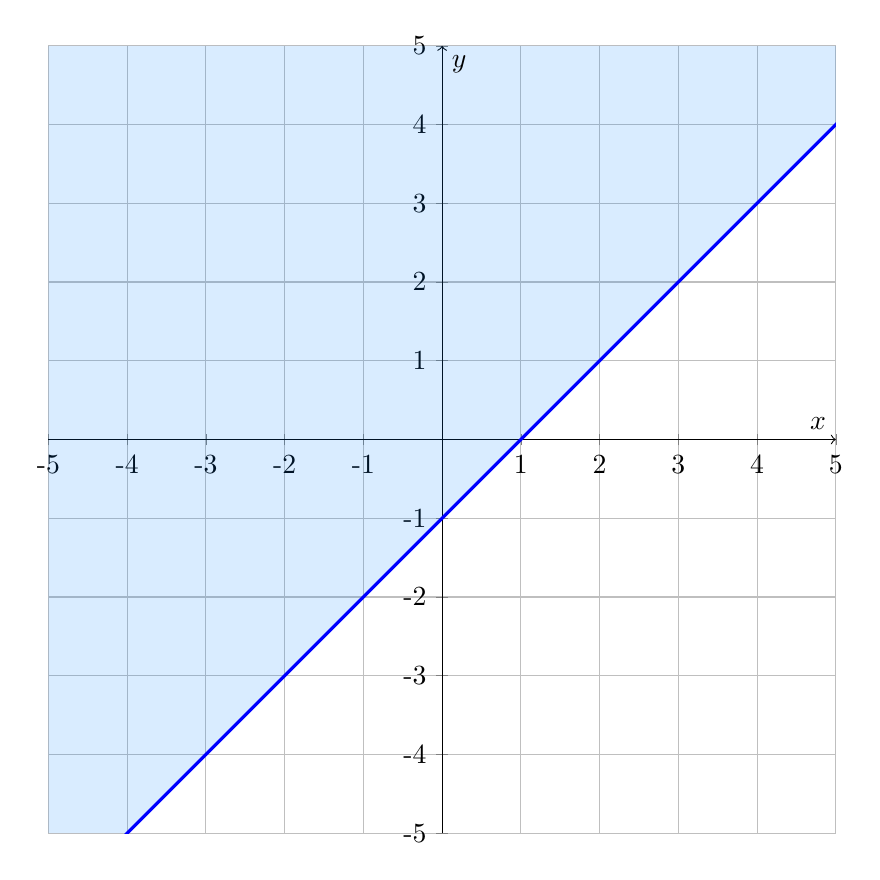
\begin{tikzpicture}
\begin{axis}[
    xmin=-5, xmax=5,
    ymin=-5, ymax=5,
    axis lines=center,
    axis on top=false,
    domain=0:1,
    x=1cm,
    y=1cm,
    xtick={-10,-9,...,10},
    xticklabels={-10,-9,...,10},
    ytick={-10,-9,...,10},
    yticklabels={-10,-9,...,10},
    axis lines=middle,
    axis line style={->},
    xlabel={$x$},
    ylabel={$y$},
    grid=major
    ]
    \addplot [thick,color=blue,fill=blue!50!cyan, 
                    fill opacity=0.15,draw opacity=0]coordinates {
            (-4,-5)
            (-5,-5)
            (-5,5)
            (5, 5)
            (5,4)  };
    \addplot [very thick,blue,domain=-10:10] {x-1};	
\end{axis}
\end{tikzpicture}
\end{center}
\end{example}

\begin{try}[http://hartleymath.com/versatilemath/tryit/\#/linear-programming--linear-inequality]
Which side of the line below should be shaded if we draw the solution set for the following inequality? \[2x+y \geq 3\]
\begin{center}
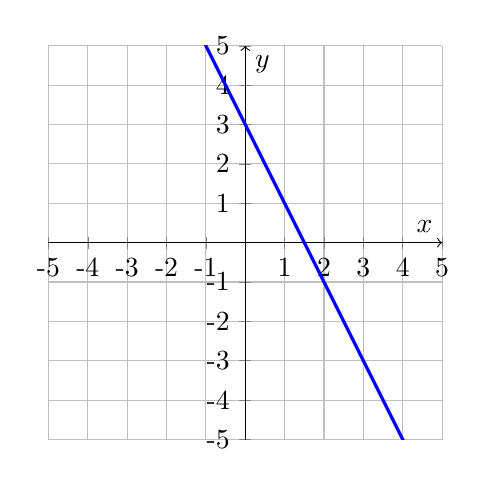
\begin{tikzpicture}
\begin{axis}[
    xmin=-5, xmax=5,
    ymin=-5, ymax=5,
    axis lines=center,
    axis on top=false,
    domain=0:1,
    x=0.5cm,
    y=0.5cm,
    xtick={-10,-9,...,10},
    xticklabels={-10,-9,...,10},
    ytick={-10,-9,...,10},
    yticklabels={-10,-9,...,10},
    axis lines=middle,
    axis line style={->},
    xlabel={$x$},
    ylabel={$y$},
    grid=major
    ]
    \addplot [very thick,blue,domain=-10:10] {-2*x+3};	
\end{axis}
\end{tikzpicture}
\end{center}
\end{try}

We picked $(0,0)$ as the test point, and we'll continue to do that whenever possible, because it makes it simple to evaluate the inequality.  The only way we wouldn't be able to use it as our test point would be if the line passed through the origin; in that case we'd simply pick another test point clearly to one side or the other of the line.

Notice that if we wrote the inequality similar to slope-intercept form, like $y \geq x-1$ in the example above, we would see that we need to shade the upper side of the line, since those are the points whose $y$-coordinates are \emph{greater} than those on the line.
\vfill
\pagebreak

\begin{example}[https://www.youtube.com/watch?v=Xw7XGKB-ado]{Graphing a Linear Inequality}
Graph the solution set for the following inequality.
\[2x-5y > 10\]

\sol
First, graph the line $2x-5y=10$.  Again, we will use the intercepts to do this:
\begin{center}
The intercepts are $(5,0)$ and $(0,-2)$
\end{center}
Since the inequality does not include 10, we draw the line dashed.
\begin{center}
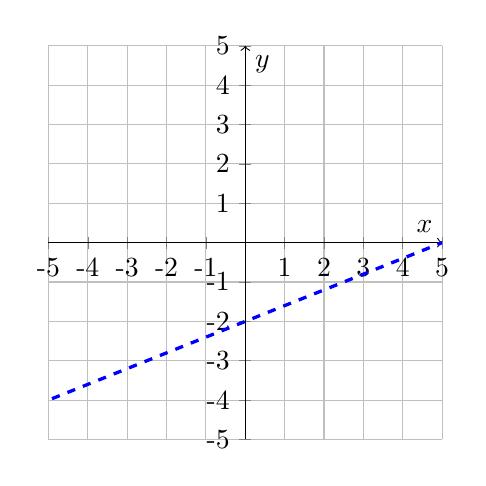
\begin{tikzpicture}
\begin{axis}[
    xmin=-5, xmax=5,
    ymin=-5, ymax=5,
    axis lines=center,
    axis on top=false,
    domain=0:1,
    x=0.5cm,
    y=0.5cm,
    xtick={-10,-9,...,10},
    xticklabels={-10,-9,...,10},
    ytick={-10,-9,...,10},
    yticklabels={-10,-9,...,10},
    axis lines=middle,
    axis line style={->},
    xlabel={$x$},
    ylabel={$y$},
    grid=major
    ]
    \addplot [very thick,blue,dashed,domain=-10:10] {(2/5)*x-2};	
\end{axis}
\end{tikzpicture}
\end{center}

To figure out which side to shade, we again pick $(0,0)$ as our test point.\\

Check $(0,0)$ in the inequality:
\begin{align*}
2x-5y &> 10\\
2(0)-5(0) &> 10
\end{align*}

This is false, so the side \emph{not} containing $(0,0)$ (the lower side) is the solution set.
\begin{center}
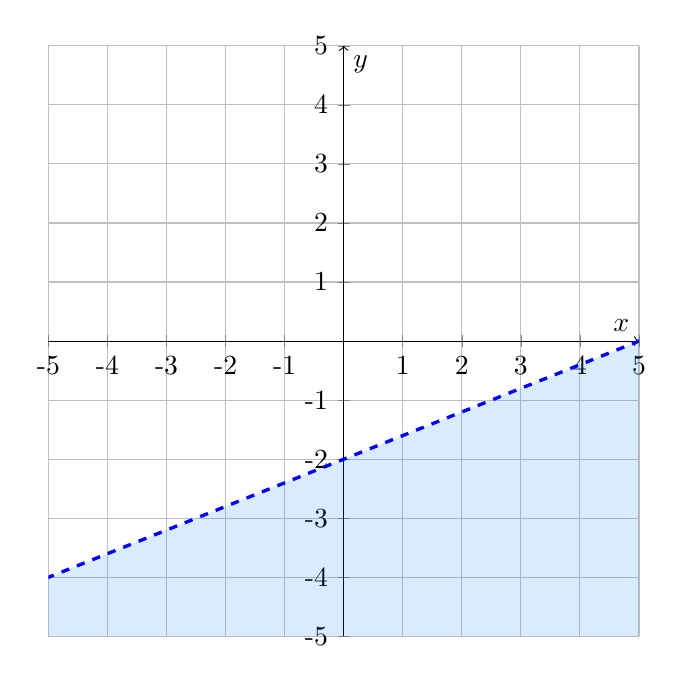
\begin{tikzpicture}
\begin{axis}[
    xmin=-5, xmax=5,
    ymin=-5, ymax=5,
    axis lines=center,
    axis on top=false,
    domain=0:1,
    x=0.75cm,
    y=0.75cm,
    xtick={-10,-9,...,10},
    xticklabels={-10,-9,...,10},
    ytick={-10,-9,...,10},
    yticklabels={-10,-9,...,10},
    axis lines=middle,
    axis line style={->},
    xlabel={$x$},
    ylabel={$y$},
    grid=major
    ]
    \addplot [thick,color=blue,fill=blue!50!cyan, 
                    fill opacity=0.15,draw opacity=0]coordinates {
            (-5,-4)
            (-5,-5)
            (5,-5)
            (5, 0)  };
    \addplot [very thick,blue,dashed,domain=-10:10] {(2/5)*x-2};	
\end{axis}
\end{tikzpicture}
\end{center}
\end{example}
\vfill
\pagebreak

\subsection{Systems of Inequalities}
What about a \emph{system} of inequalities?  When it comes to the optimization problems, we'll have several inequalities, and we'll want to know what values satisfy \emph{all} of them at once.  Just like the solution to a system of equations is the point that lies on both lines--the place where the two lines overlap--the solution set for a system of inequalities is the \emph{overlap} of the individual solution sets.

\begin{proc}{Solutions to a System of Linear Inequalities}
The solutions to a system of inequalities are the points that lie in the region where the solution sets of the individual inequalities overlap.
\end{proc}

For instance, suppose we had two inequalities whose individual solution sets looked like the ones below.
\begin{center}
\begin{tabular}{c c}
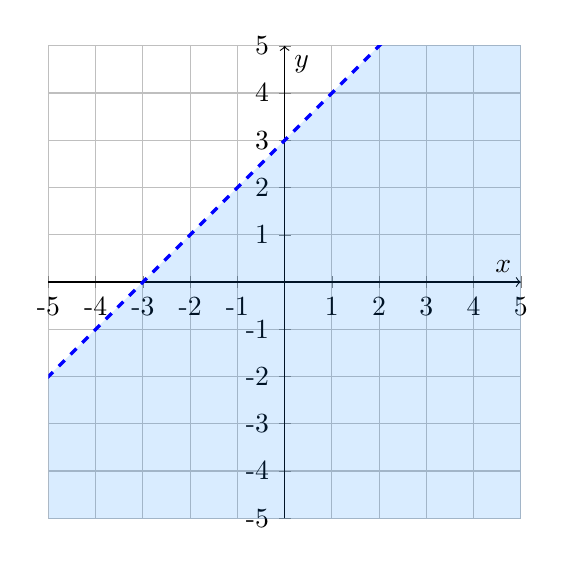
\begin{tikzpicture}
\begin{axis}[
    xmin=-5, xmax=5,
    ymin=-5, ymax=5,
    axis lines=center,
    axis on top=false,
    domain=0:1,
    x=0.6cm,
    y=0.6cm,
    xtick={-10,-9,...,10},
    xticklabels={-10,-9,...,10},
    ytick={-10,-9,...,10},
    yticklabels={-10,-9,...,10},
    axis lines=middle,
    axis line style={->},
    xlabel={$x$},
    ylabel={$y$},
    grid=major
    ]
	\addplot [thick,color=blue,fill=blue!50!cyan, 
                    fill opacity=0.15,draw opacity=0]coordinates {
            (7, 10)
            (10,10)
            (10,-10)
            (-10,-10)
            (-10, -7)  };
	\addplot [very thick,blue,dashed,domain=-10:10] {x+3};
\end{axis}
\end{tikzpicture}
&
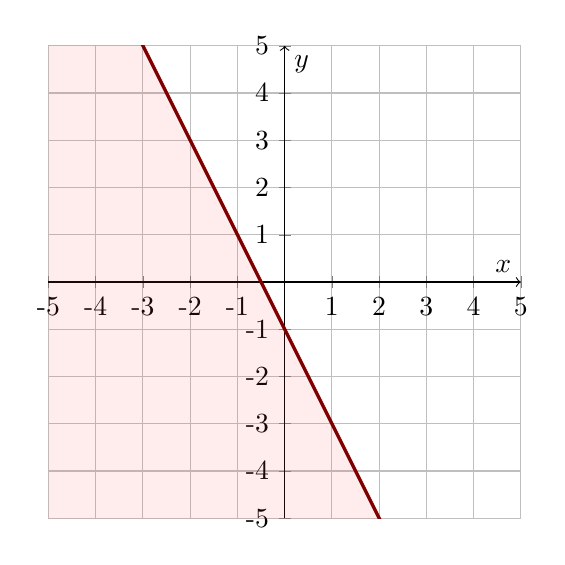
\begin{tikzpicture}
\begin{axis}[
    xmin=-5, xmax=5,
    ymin=-5, ymax=5,
    axis lines=center,
    axis on top=false,
    domain=0:1,
    x=0.6cm,
    y=0.6cm,
    xtick={-10,-9,...,10},
    xticklabels={-10,-9,...,10},
    ytick={-10,-9,...,10},
    yticklabels={-10,-9,...,10},
    axis lines=middle,
    axis line style={->},
    xlabel={$x$},
    ylabel={$y$},
    grid=major
    ]
    \addplot [thick,color=blue,fill=red!70!white, 
                    fill opacity=0.1,draw opacity=0]coordinates {
            (-11/2, 10) 
            (9/2, -10)
            (-10,-10)
            (-10, 10)  };
	\addplot [very thick,red!50!black,domain=-10:10] {-2*x-1};
\end{axis}
\end{tikzpicture}
\end{tabular}
\end{center}
We could draw them on the same graph, and the combined solution set would be the overlapping region.
\begin{center}
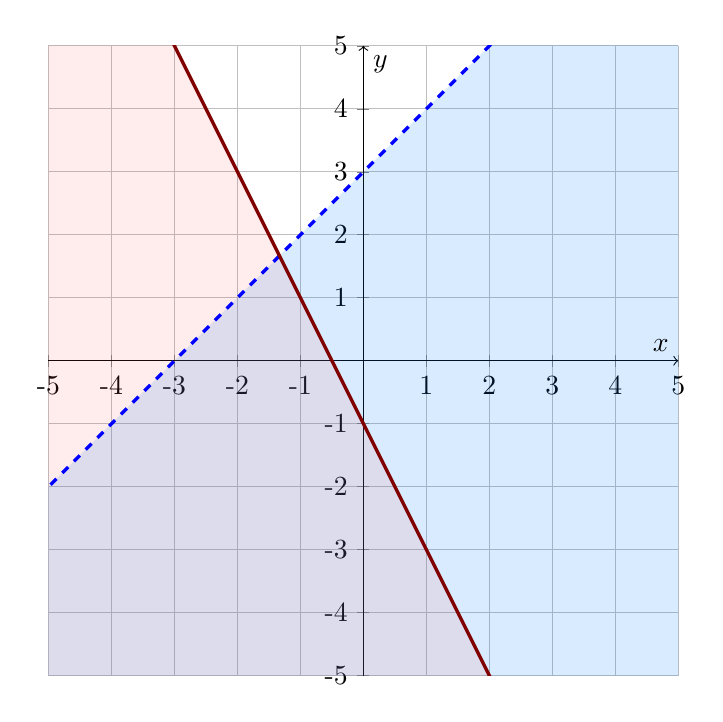
\begin{tikzpicture}
\begin{axis}[
    xmin=-5, xmax=5,
    ymin=-5, ymax=5,
    axis lines=center,
    axis on top=false,
    domain=0:1,
    x=0.8cm,
    y=0.8cm,
    xtick={-10,-9,...,10},
    xticklabels={-10,-9,...,10},
    ytick={-10,-9,...,10},
    yticklabels={-10,-9,...,10},
    axis lines=middle,
    axis line style={->},
    xlabel={$x$},
    ylabel={$y$},
    grid=major
    ]
	\addplot [thick,color=blue,fill=blue!50!cyan, 
                    fill opacity=0.15,draw opacity=0]coordinates {
            (7, 10)
            (10,10)
            (10,-10)
            (-10,-10)
            (-10, -7)  };
    \addplot [thick,color=blue,fill=red!70!white, 
                    fill opacity=0.1,draw opacity=0]coordinates {
            (-11/2, 10) 
            (9/2, -10)
            (-10,-10)
            (-10, 10)  };
	\addplot [very thick,blue,dashed,domain=-10:10] {x+3};
	\addplot [very thick,red!50!black,domain=-10:10] {-2*x-1};
\end{axis}
\end{tikzpicture}
\end{center}
\pagebreak

We can redraw the picture with only the overlapping region shaded, to make it clearer.
\begin{center}
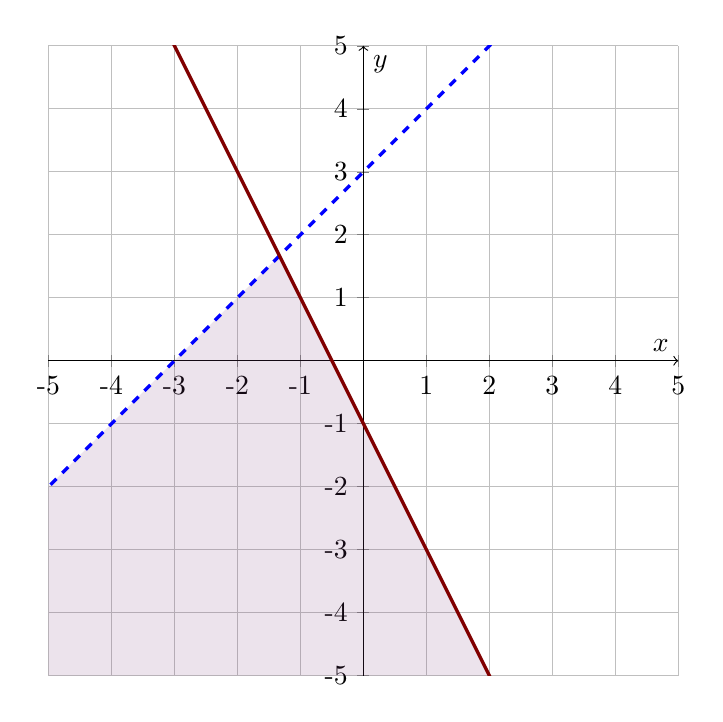
\begin{tikzpicture}
\begin{axis}[
    xmin=-5, xmax=5,
    ymin=-5, ymax=5,
    axis lines=center,
    axis on top=false,
    domain=0:1,
    x=0.8cm,
    y=0.8cm,
    xtick={-10,-9,...,10},
    xticklabels={-10,-9,...,10},
    ytick={-10,-9,...,10},
    yticklabels={-10,-9,...,10},
    axis lines=middle,
    axis line style={->},
    xlabel={$x$},
    ylabel={$y$},
    grid=major
    ]
	\addplot [thick,color=blue,fill=blue!50!cyan!50!red, 
                    fill opacity=0.15,draw opacity=0]coordinates {
            (-5, -2)
            (-4/3,5/3)
            (2,-5)
            (-5,-5) };   
	\addplot [very thick,blue,dashed,domain=-10:10] {x+3};
	\addplot [very thick,red!50!black,domain=-10:10] {-2*x-1};
\end{axis}
\end{tikzpicture}
\end{center}

This illustrates how we graph the solution set for a system of linear inequalities: simply graph the solution set for each inequality and see where they overlap.

\begin{example}[https://www.youtube.com/watch?v=8VWlVARcFWU]{Graphing for a System of Inequalities}
Graph the solution set for the following system of inequalities.
\begin{align*}
2x+y &< 4\\
x-y &> 4
\end{align*}

\sol
We begin by graphing the two corresponding lines, using the intercepts to graph.  Note that both inequalities do \emph{not} include equality, so we draw both lines dashed.
\begin{center}
\begin{longtable}{c c c}
$2x+y = 4$ & and & $x-y=4$\\
& & \\
\begin{tabular}{c | c}
$x$ & $y$\\
\hline
0 & 4\\
2 & 0
\end{tabular}
& &
\begin{tabular}{c c}
$x$ & $y$\\
\hline
0 & $-4$\\
4 & 0
\end{tabular}\\
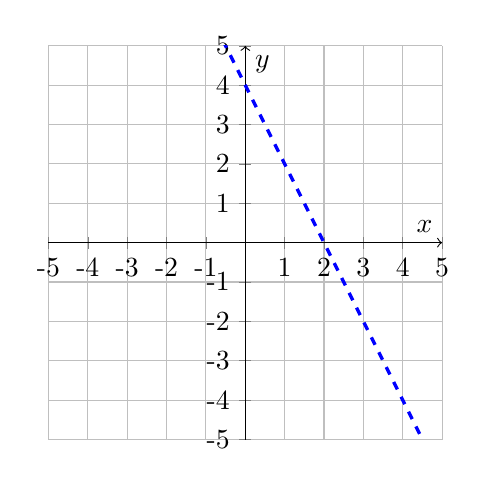
\begin{tikzpicture}
\begin{axis}[
    xmin=-5, xmax=5,
    ymin=-5, ymax=5,
    axis lines=center,
    axis on top=false,
    domain=0:1,
    x=0.5cm,
    y=0.5cm,
    xtick={-10,-9,...,10},
    xticklabels={-10,-9,...,10},
    ytick={-10,-9,...,10},
    yticklabels={-10,-9,...,10},
    axis lines=middle,
    axis line style={->},
    xlabel={$x$},
    ylabel={$y$},
    grid=major
    ]
	\addplot [very thick,blue,dashed,domain=-10:10] {-2*x+4};
\end{axis}
\end{tikzpicture}
& &
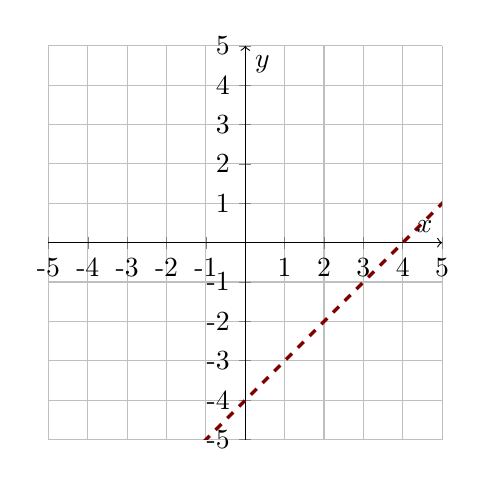
\begin{tikzpicture}
\begin{axis}[
    xmin=-5, xmax=5,
    ymin=-5, ymax=5,
    axis lines=center,
    axis on top=false,
    domain=0:1,
    x=0.5cm,
    y=0.5cm,
    xtick={-10,-9,...,10},
    xticklabels={-10,-9,...,10},
    ytick={-10,-9,...,10},
    yticklabels={-10,-9,...,10},
    axis lines=middle,
    axis line style={->},
    xlabel={$x$},
    ylabel={$y$},
    grid=major
    ]
	\addplot [very thick,red!50!black,dashed,domain=-10:10] {x-4};
\end{axis}
\end{tikzpicture}\\
\multicolumn{3}{l}{Next, test the origin on each inequality to see which side to shade:}\\
$2(0)+0<4$ & & $0-0>4$\\
TRUE & & FALSE\\
& & \\
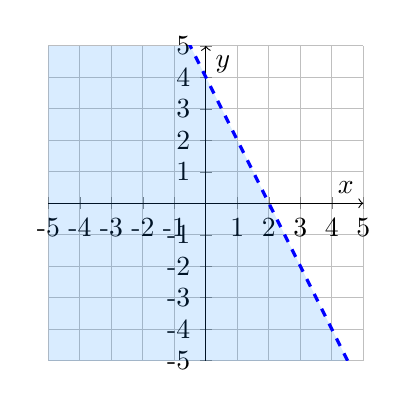
\begin{tikzpicture}
\begin{axis}[
    xmin=-5, xmax=5,
    ymin=-5, ymax=5,
    axis lines=center,
    axis on top=false,
    domain=0:1,
    x=0.4cm,
    y=0.4cm,
    xtick={-10,-9,...,10},
    xticklabels={-10,-9,...,10},
    ytick={-10,-9,...,10},
    yticklabels={-10,-9,...,10},
    axis lines=middle,
    axis line style={->},
    xlabel={$x$},
    ylabel={$y$},
    grid=major
    ]
    \addplot [thick,color=blue,fill=blue!50!cyan, 
                    fill opacity=0.15,draw opacity=0]coordinates {
            (-1/2, 5)
            (-5,5)
            (-5,-5)
            (4.5,-5)  };
	\addplot [very thick,blue,dashed,domain=-10:10] {-2*x+4};
\end{axis}
\end{tikzpicture}
& &
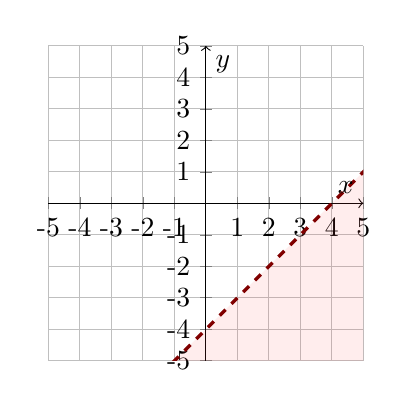
\begin{tikzpicture}
\begin{axis}[
    xmin=-5, xmax=5,
    ymin=-5, ymax=5,
    axis lines=center,
    axis on top=false,
    domain=0:1,
    x=0.4cm,
    y=0.4cm,
    xtick={-10,-9,...,10},
    xticklabels={-10,-9,...,10},
    ytick={-10,-9,...,10},
    yticklabels={-10,-9,...,10},
    axis lines=middle,
    axis line style={->},
    xlabel={$x$},
    ylabel={$y$},
    grid=major
    ]
    \addplot [thick,color=blue,fill=red!70!white, 
                    fill opacity=0.1,draw opacity=0]coordinates {
            (-1, -5) 
            (5, -5)
            (5,1)  };
	\addplot [very thick,red!50!black,dashed,domain=-10:10] {x-4};
\end{axis}
\end{tikzpicture}\\
\end{longtable}
\end{center}

Finally, combine the pictures (we'll draw the final product with only the overlapping region shaded):
\begin{center}
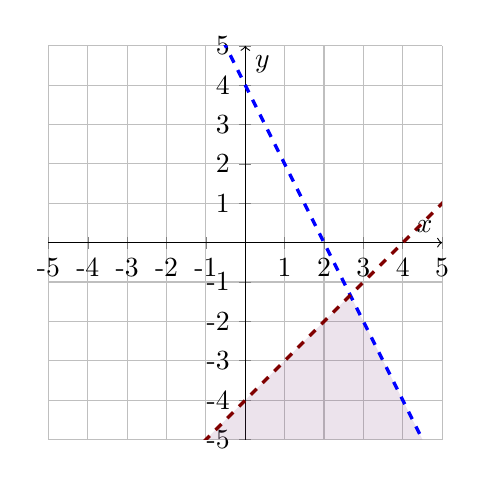
\begin{tikzpicture}
\begin{axis}[
    xmin=-5, xmax=5,
    ymin=-5, ymax=5,
    axis lines=center,
    axis on top=false,
    domain=0:1,
    x=0.5cm,
    y=0.5cm,
    xtick={-10,-9,...,10},
    xticklabels={-10,-9,...,10},
    ytick={-10,-9,...,10},
    yticklabels={-10,-9,...,10},
    axis lines=middle,
    axis line style={->},
    xlabel={$x$},
    ylabel={$y$},
    grid=major
    ]
	\addplot [thick,color=blue,fill=blue!50!cyan!50!red, 
                    fill opacity=0.15,draw opacity=0]coordinates {
            (-1, -5)
            (4.5,-5)
            (8/3,-4/3) };   
	\addplot [very thick,blue,dashed,domain=-10:10] {-2*x+4};
	\addplot [very thick,red!50!black,dashed,domain=-10:10] {x-4};
\end{axis}
\end{tikzpicture}
\end{center}
\end{example}

\begin{try}[http://hartleymath.com/versatilemath/tryit/\#/linear-programming--system-of-linear-inequalities]
Is the graph below correct for the following system of inequalities?  If not, what is wrong with it?
\begin{align*}
x+y &\leq 4\\
y &> 2x-4
\end{align*}

\begin{center}
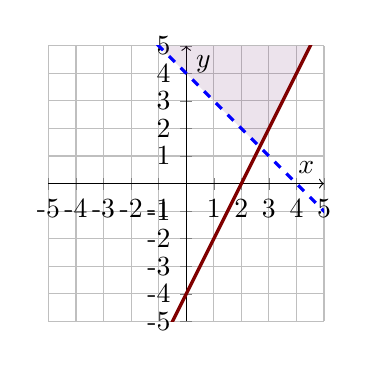
\begin{tikzpicture}
\begin{axis}[
    xmin=-5, xmax=5,
    ymin=-5, ymax=5,
    axis lines=center,
    axis on top=false,
    domain=0:1,
    x=0.35cm,
    y=0.35cm,
    xtick={-10,-9,...,10},
    xticklabels={-10,-9,...,10},
    ytick={-10,-9,...,10},
    yticklabels={-10,-9,...,10},
    axis lines=middle,
    axis line style={->},
    xlabel={$x$},
    ylabel={$y$},
    grid=major
    ]
	\addplot [thick,color=blue,fill=blue!50!cyan!50!red, 
                    fill opacity=0.15,draw opacity=0]coordinates {
            (-1, 5)
            (4.5,5)
            (8/3,4/3) };   
	\addplot [very thick,blue,dashed,domain=-10:10] {-x+4};
	\addplot [very thick,red!50!black,domain=-10:10] {2*x-4};
\end{axis}
\end{tikzpicture}
\end{center}
\end{try}